% Copyright 2007 by Till Tantau
%
% This file may be distributed and/or modified
%
% 1. under the LaTeX Project Public License and/or
% 2. under the GNU Public License.
%
% See the file doc/licenses/LICENSE for more details.


\lecture[23]{The least-squares line}{lecture-text}

\subtitle{and the correlation coefficient}

\date{24 November 2015}

% pp. 492-505


\begin{document}

\begin{frame}
  \maketitle
\end{frame}



\begin{frame}{Last time}
  \begin{enumerate}
      \item The \alert{correlation coefficient}, $r$,
      \item measures the strength of a linear relationship between two quantitative variables.
      \item It can be transformed to have a $t$ distribution
      \item under the null hypothesis of $r=0$ (no linear relationship).
  \end{enumerate}

    \vspace{2em}

    \structure{Today:} other ways to think about it.

\end{frame}

\begin{frame}\frametitle<presentation>{Outline}
  \tableofcontents
\end{frame}


\section{Prediction and line--fitting}


%%%%%%
\begin{frame}{Example:}
    Monthly mean minimum \& maximum temperatures
    at USC, 1906--1997  (1196 data points),
    \uncover<2->{with monthly means before 1920 subtracted}
    \begin{center}
    \includegraphics<1>{usc-temps.pdf}
    \includegraphics<2>{usc-temps-stdized.pdf}
    \end{center}

    \pause
    \vspace{2em}

    \begin{align*}
        r&=0.1582157 \\
        n&=1196 \\
        t_s &= r \sqrt{\frac{n-2}{1-r^2}} = 5.536772 
    \end{align*}
    and with $df=1194$, $P=3.79\times 10^{-8}$.

\end{frame}

\subsection{the SD line}

%%%%%%
\begin{frame}{Which line?}

    There are \structure{several reasons} to put a straight line through bivariate data:
    \begin{enumerate}
        \item visual emphasis
        \item quantitative description of the mean relationship \\
            (slope, intercept)
        \item prediction of $Y$ for new values of $X$
    \end{enumerate}


    \vspace{2em}

    \structure{Example:} interpolate temperatures for 1915--1920
    \begin{center}
    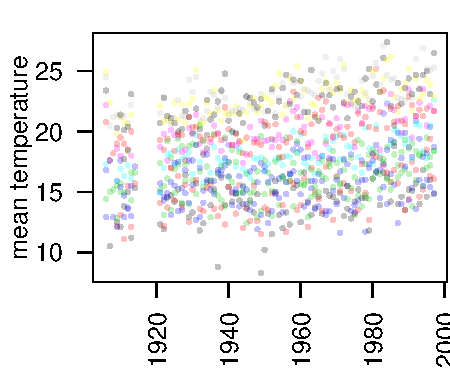
\includegraphics[width=.5\textwidth]{usc-temps.pdf}
    \end{center}

\end{frame}


%%%%%%
\begin{frame}{The SD line}

    One possible line is the \alert{SD line},
    that
    \begin{itemize}
        \item goes through the means $(\bar x, \bar y)$, and
        \item has slope $\pm s_y/s_x$.
    \end{itemize}
    (i.e.\ is $y=x$ on the plot of $z$-scores)

    \vspace{1em}

    \structure{Example:} \uncover<3->{with yearly means}

    \centering
    \includegraphics<2>{usc-temps-lines}
    \includegraphics<3>{usc-temps-lines-means}

\end{frame}

\subsection{the Regression Line}

%%%%%%
\begin{frame}{The line of Local Averages}

    \structure{Instead}, fit a model with a \alert{linear relationship \\ \hspace{3em} for the conditional mean of $Y$}
    \begin{align*}
        Y &= \beta_0 + \beta_1 X + \epsilon, \\
        \uncover<2->{\text{so} \quad \mu_{Y|X} &= \beta_0 + \beta_1 X ,}
    \end{align*}
    i.e.\ the mean value of $Y$ is linear in $X$.
    

    \begin{center}
        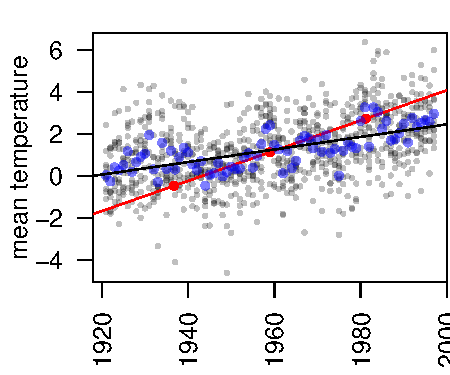
\includegraphics{usc-temps-both-lines}
    \end{center}

\end{frame}


%%%%%%
\begin{frame}{Relationship to $r$}

    The line of local averages,
    a.k.a.\ the \alert{regression line}
    has 
    \begin{align*}
        \text{(slope)}\quad b_1 &= r \; \frac{s_y}{s_x} \\
        \text{(intercept)}\quad b_0 &= \bar y - b_1 \bar x,
    \end{align*}
    i.e.\ slope $r$ in normalized coordinates,
    and passing through $(\bar x, \bar y)$.

    \vspace{2em}

    Our estimate of the mean of $Y$ given $X$ is then
    \[
        \hat \mu_{Y|X} = b_0 + b_1 X .
    \]

\end{frame}

%%%%%%
\begin{frame}{Example:}

    \centering
        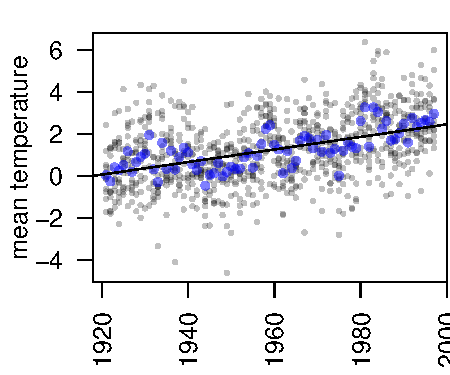
\includegraphics{usc-temps-regression}

    \begin{align*}
        \bar x &= 1966.917 & s_x &= 26.81045 \\
        \bar y &= 1.155366 & s_y &= 1.550648 \\
               r &= 0.3128291 & \hat \mu_{Y|X} &= 0.018 \; X - 33.8 .
    \end{align*}

\end{frame}

\section{Sums of squares}

\subsection{Residuals}


%%%%%%
\begin{frame}{Conclusions?}

    \begin{center}
        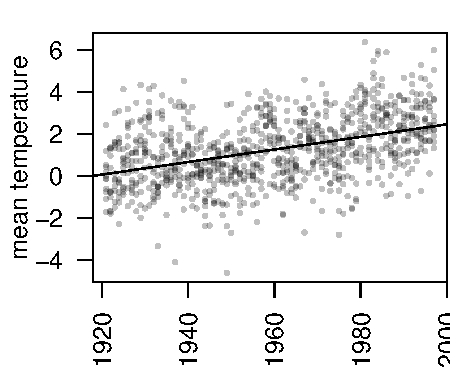
\includegraphics[height=2in]{usc-temps-just-regression}

    \begin{align*}
        r &= 0.3128291 & n &= 1114 \\
        t_s &=  r \sqrt{ \frac{ n-2}{1-r^2} } = 10.98305 &
        P &< 10^{-16} .
    \end{align*}
    What do we conclude?

    \end{center}
\end{frame}


%%%%%%
\begin{frame}{Observed minus predicted}

    \begin{block}{Residuals}
        The residuals of a regression are the differences between the \structure{observed values} 
        and the \structure{predicted values},
        i.e.\ the vertical distances to the regression line,
        or the \alert{errors} we'd make if we predicted with the regression line.
    \end{block}

    \vspace{2em}

    Predicted:
    \[
        \hat y_i = b_0 + b_1 x_i
    \]
    Residual, or error:
    \[
        e_i = y_i - \hat y_i .
    \]

\end{frame}


%%%%%%
\begin{frame}{Residual sum of squares}

    \begin{block}{$\SS(\text{resid})$}
        The \alert{residual sum of squares} is the sum of the squares of the residuals:
        \[
            \SS(\text{resid}) = \sum_i (y_i - \hat y_i)^2 = \sum_i e_i^2 .
        \]
    \end{block}

    \vspace{2em}

    The regression line, or the line of local averages, is also known as the \structure{least squares regression line},\\
    which is the straight line that \alert{minimizes} $\SS(\text{resid})$.

    \vspace{2em}

    Amazing fact: the equation of this line is easy to compute,
    and is related to the correlation coefficient. \\
    (i.e.\ the equations for $b_0$ and $b_1$ earlier)


\end{frame}


%%%%%%
\begin{frame}{Residual SD}

    \begin{block}{$s_e$}
        The \alert{residual standard deviation} is
        \[ s_e = \sqrt{ \frac{ \sum (y_i - \hat y_i)^2 }{n-2} } = \sqrt{ \frac{ \SS(\text{resid}) }{ n-2 } } .  \]
    \end{block}

    \vspace{2em}

    This measures the spread of the points about the regression line.


\end{frame}


%%%%%%
\begin{frame}{Example:}
    \centering
        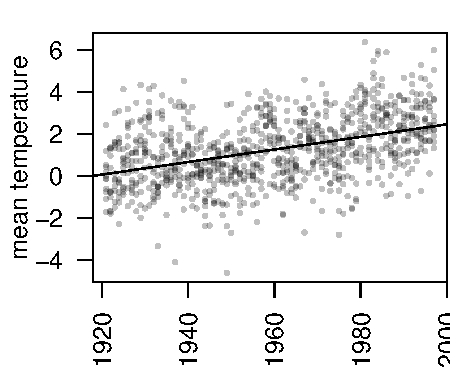
\includegraphics{usc-temps-just-regression}

    \begin{align*}
       r &= 0.3128291 \\
        s_e &= 2.110126 .
    \end{align*}


\end{frame}


%%%%%%
\begin{frame}{Partitioning sums of squares}

    Often, people report $r^2$ as the ``\alert{proportion of variance explained}'':
    \[
        r^2 = 1 - (1-\frac{1}{n-1}) \frac{s_e^2}{s_y^2} \approx 1 - \frac{s_e^2}{s_y^2}.
    \]

    \pause

    \only<1-2>{
\centering
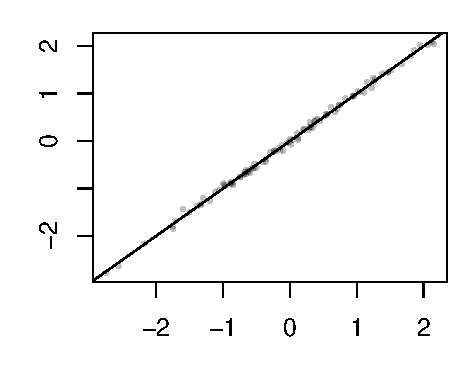
\includegraphics[height=2in]{r2ex-1.pdf}
        \[ r^2 = 0.9975455 \]
    }

    \only<3>{
\centering
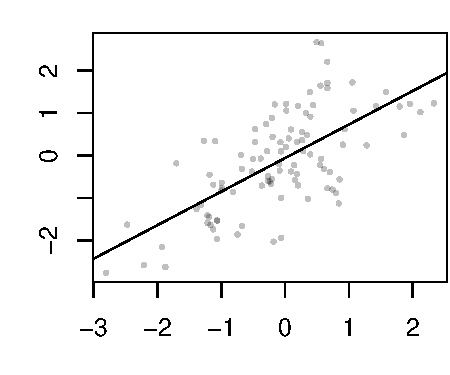
\includegraphics[height=2in]{r2ex-2.pdf}
        \[ r^2 = 0.4406095 \]
    }

    \only<4>{
\centering
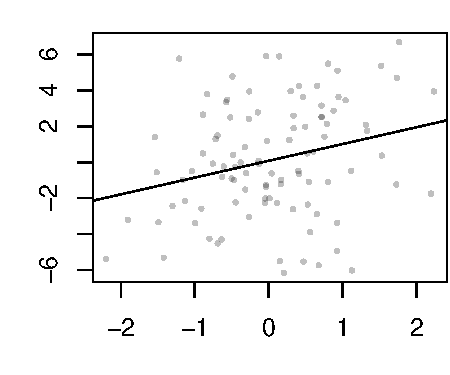
\includegraphics[height=2in]{r2ex-3.pdf}
        \[ r^2 = 0.06929872 \]
    }

\end{frame}


\section{Examples}



%%%%%%
\begin{frame}{From the book}

  \begin{center}
  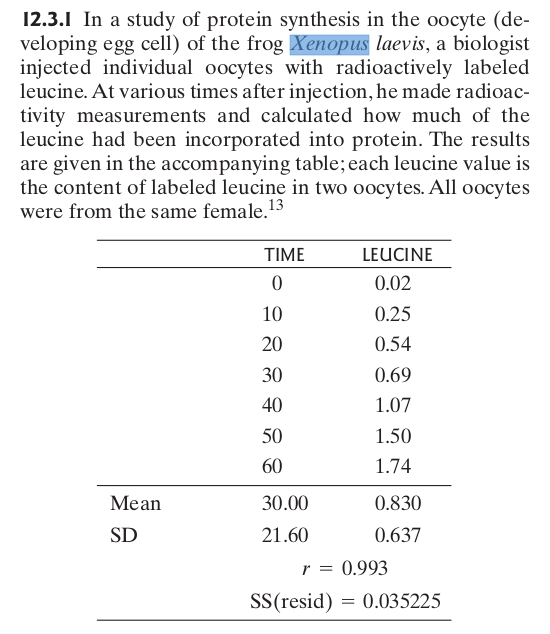
\includegraphics[height=.8\textheight]{ex12-3-1.png}
  \end{center}

\end{frame}


%%%%%%
\begin{frame}{From the wild}


  \begin{quote}
    1. Residents of a chronic care hospital (13 men of mean age 88.5 +/- 6 SD years and 13 women of mean age 86.5 +/- 6 SD years) who had multiple pathologies were assessed for leg extensor capability in several ways. 2. A custom-built rig was used to assess leg extensor power, that is, maximal power output over less than 1 s in a single extension of one leg. Performance measures were obtained by timing chair rises, stair climbing,  and a walk. \ldots 3. Leg extensor power was \textbf{significantly correlated} with all performance measures, but the performance measures were not related to each other except for chair rising and walking speed. 4. Women had significantly less extensor power than men, but their power explained more of the variance in performance, e.g.\ power \textbf{accounted for 86\% of the variance} in walking speed.
  \end{quote}
  \figcaption{ Leg extensor power and functional performance in very old men and women, Bassey et al 1992 }

\end{frame}

% . . . 



%%%%%%
\begin{frame}{Conditional means, SDs}

  \begin{block}{Notation}
    \begin{align*}
      \mu_{Y|X} &= \; \text{mean value of $Y$ given $X$} \\
      \sigma_{Y|X} &= \; \text{SD of $Y$ given $X$} \\
    \end{align*}
  \end{block}


    \vspace{2em}

    \structure{Example:}
    Drug dose ($X$) and blood pressure ($Y$) in patients. \\
    $\mu_{Y|X}$ is the mean blood pressure among patients with dose $X$; \\
    $\sigma_{Y|X}$ is the SD.

\end{frame}

%%%%%%
\begin{frame}{The linear model}

  \structure{In words,} the values of $Y$ are normally distributed with mean
  a linear function of $X$ and a standard deviation that does not depend on $X$:
  \begin{align*}
    \mu_{Y|X} &= \beta_0 + \beta_1 X \\
    \sigma_{Y|X} &= \sigma_\epsilon
  \end{align*}
  or, equivalently,
  \begin{align*}
    Y = \beta_0 + \beta_1 X + \epsilon \\
    \epsilon \; \text{independent, with SD $\sigma_\epsilon$} .
  \end{align*}

\end{frame}


%%%%%%
\begin{frame}{Why linear?}

  \begin{enumerate}
      
    \item It is arguably the simplest possible relationship between $X$ and $Y$,
      requiring only two parameters ($b_0$ and $b_1$)

    \item Most things look linear at the right level of approximation.

    \item The mathematics works out nicely.

    \item Nonlinear relationships can often be transformed to linear relationships.

  \end{enumerate}

\end{frame}


\section<article>{Summary}
\section<presentation>*{Summary}

\begin{frame}{Summary}
  \begin{enumerate}
      \item The \alert{least-squares regression line}
      \item goes through the means (center of mass)
      \item and has slope equal to the regression coefficient $r$ in normalized ($z$-score) coordinates.
      \item This line \alert{also} gives the conditional mean value of $Y$ given $X$.
      \item The residual SD measures the spread of the data about the regression line.
  \end{enumerate}
\end{frame}

% homework
\begin{frame}{Homework}
  \begin{center}


  12.3.3

  \vspace{2em}

  12.3.6

  \end{center}
\end{frame}


\end{document}





